\chapter{Introduction}
\label{chap:Introduction}

\section{Background}

Modern rail vehicles like trains, metro vehicles or trams have to meet ever increasing acoustic requirements and regulations not only to improve the acoustic comfort of the passengers, but also to reduce environmental noise pollution from railways \cite{paozalyte_pollution_2011, li_25d_2021, zhang_sound_2019}.

The transmisson of noises is complex procedures because many paths: airborne, structure borne structural vibration


- outline the specific objective of the research
The aim of this thesis is ...

This thesis aims to provide/determine/develop/investigate

- Provide overview of thesis structure:
The thesis is structured as follow ...


\begin{figure}[H]
    \centering
    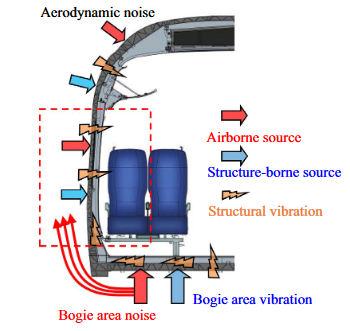
\includegraphics[width=0.6\textwidth]{fig/noise_transmission_path.png}
    \caption{Transmission path of exterior noise sources \cite{zhang_sound_2019}}
    \label{fig:my_label}
\end{figure}

\newpage
\section{Aims and objectives}

This thesis, in collaboration with Siemens Mobility Austria GmbH, aims to develop a finite-element model suitable for predicting the sound propagation from train underfloor area into the exterior environment around the carbody. 


The thesis is organised as follows. The fundamental background of the thesis is explained in Chap. \ref{chap:Theory}. Chap. \ref{chap:measurement} describes the outer pressure field measurement